\section{Background}
\label{sec:back}

This section reviews the main concepts and approaches related to lockstep execution relevant for this work.

\subsection{Redundancy, Diversity and Sphere of Replication}
The design, as well as the verification and validation (V\&V) stages for safety-related systems arguably remove unreasonable risk of any kind of systematic fault, either software or hardware related. However, random hardware faults are unavoidable in nature, so they must be managed with suitable safety measures, being diverse redundancy a mandatory safety measure for the highest Safety Integrity Levels (SIL for short).

Diverse redundancy can be realized by using diverse hardware and/or software, but these approaches may double part of the design, and V\&V costs. Alternatively, diverse redundancy can also be realized by executing the same software in identical hardware, but with some staggering, hence guaranteeing that replicas hold different state at any time instant so that any common fault will lead to diverse errors (if any). This approach, if realized with two cores, is referred to as Dual Core LockStepping (DCLS) and is used in several commercial processors~\cite{infineon_aurix,STlockstep,RendundancyASILD}.

The sphere of replication determines what outputs of the replicas are compared to detect errors. In the case of hardware-based lockstep, such sphere includes only a core, so any off-core activity (data fetch or store beyond in-core caches, I/O activity, interrupts, etc.) is compared across cores for error detection. In the case of light-weight lockstep execution, it is limited to programs or code regions without I/O, and detects errors by comparing data outputs at the end of the execution.


\subsection{Lockstep Schemes}

\begin{figure}[t!]
\centering
\begin{tabular}{cc}
  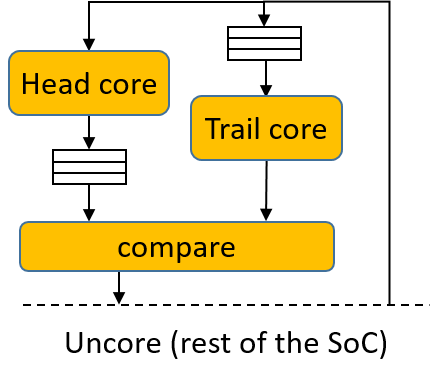
\includegraphics[width=0.37\columnwidth]{imgs/HWlockstep.png} & 
  
\includegraphics[width=0.53\columnwidth]{imgs/SWlockstep.png} \\
  (a) Hardware-only & (b) Software-only \\
\end{tabular}
  \caption{Schematic of the existing lockstep schemes.}
  \label{fig:HWSWlockstep}
\end{figure}

\textbf{Tight hardware-based lockstep execution}. This approach, implemented in processors such as, for instance, the Infineon AURIX family~\cite{infineon_aurix}, uses two physical cores (head and trail cores) out of which only one (e.g., head core) is visible at user level and the other one (e.g., trail core) is a shadow core. They perform \emph{exactly} the same activity but shifted by $N$ cycles, 
so that the state of the trail core matches that of the head core $N$ cycles before.
External requests (data load/store, interrupts, etc.) are compared before being exposed externally, hence needing some buffering to store head requests during $N$ cycles. Analogously, responses are delivered immediately to the head core when they arrive, but queued during $N$ cycles before being delivered to the trail core, which also needs some buffering. Such scheme is depicted in Figure~\ref{fig:HWSWlockstep}(a). Note that staggering is typically low (e.g., 2 or 3 cycles) to keep buffering overheads low.

\textbf{Light-weight software-based lockstep execution}. In this approach, redundancy is created at software level by running a given program (task) twice on different cores~\cite{SergiDFT}. Those task replicas run along with a monitor thread, which is deployed in a third core, to enforce some staggering across replicas so that one of them becomes the head and the other one the trail task (and core). Note that the monitor itself is unprotected, so this approach requires the execution of the monitor to occur on a core with hardware-based lockstepping, either in the same or another chip. 
In detail, the operation of this scheme is as follows (see Figure~\ref{fig:HWSWlockstep}(b)): the monitor schedules redundant processes (replicas) in two different cores, but only allows the head core to make progress. The monitor collects the number of instructions executed by each core ($\#instr$ in the figure), and only allows the trail core to execute its task if $\#instr_{head} - \#instr_{trail}$, namely the staggering in terms of number of instructions, exceeds a given threshold $TH_{stag}$. Such condition is checked by the monitor every $T_{check}$ cycles to decide whether the trail core is allowed to proceed during the following interval. Only when the head core finishes its execution, the trail core is allowed to run unrestrictedly. Results from both executions are compared when both cores complete their execution. 
Note that between two consecutive checks of the staggering, the trail core could execute up to $T_{check} \cdot CommitWidth$ instructions, where $CommitWidth$ stands for the maximum number of instructions that can be retired per cycle. $TH_{stag}$ must be strictly higher than $T_{check} \cdot CommitWidth$.
As shown in \cite{SergiDFT}, due to the software overheads to collect $\#instr_{head}$ and $\#instr_{trail}$, and to stall a process -- if needed, $TH_{stag}$ must be a number of instructions taking at least around 100$\mu$s to run.
